\documentclass{beamer}
%[aspectratio=169]   \usepackage[czech]{babel}
\usepackage{apo-lecture-cz}
\usepackage{pdfpages}
\usepackage{pdfcomment}
\usepackage{listings}

\subtitle{Lekce 04. Central Processing Unit (CPU)}
\author{Pavel Píša\\ \small\texttt{pisa@fel.cvut.cz}}
\begin{document}

\maketitle

\section{Simulátor}

\begin{frame}
\frametitle{QtMips and QtRVSim – Origin and Development}

\begin{itemize}
\item MipsIt used in past for Computer Architecture course at the Czech Technical University in Prague, Faculty of Electrical Engineering
\item Diploma theses of Karel Kočí mentored by Pavel Píša
Graphical CPU Simulator with Cache Visualization
https://dspace.cvut.cz/bitstream/handle/10467/76764/F3-DP-2018-Koci-Karel-diploma.pdf
\item Switch to QtMips in the 2019 summer semester
\item Fixes, extension and partial internals redesign by Pavel Píša
\item Switch to RISC-V architecture in 2022. Main work by Jakub Dupák 2021
Graphical RISC-V Architecture Simulator - Memory Model and Project Management
\item https://dspace.cvut.cz/bitstream/handle/10467/94446/F3-BP-2021-Dupak-Jakub-thesis.pdf

\item Alternatives:
\begin{itemize}
 \item RARS: IDE with detailed help and hints
 https://github.com/TheThirdOne/rars
 \item EduMIPS64: 1x fixed and 3x FP pipelines
 https://www.edumips.org/
\end{itemize}
\end{itemize}

\end{frame}


\begin{frame}
\frametitle{QtRVSim - Download}
\begin{itemize}
\item Windows, Linux, Mac
https://github.com/cvut/qtrvsim/releases
\item  Ubuntu
https://launchpad.net/~qtrvsimteam/+archive/ubuntu/ppa
\item Suse, Fedora and Debian
https://software.opensuse.org/download.html?project=home%3Ajdupak&package=qtrvsim
\item Suse Factory
TBD
\item Online version
https://dev.jakubdupak.com/qtrvsim/
\item LinuxDays 2019 QtMips talk – Record of Interactive Session
https://youtu.be/fhcdYtpFsyw
https://pretalx.linuxdays.cz/2019/talk/EAYAGG/
\end{itemize}
\end{frame}

\begin{frame}
\frametitle{John von Neumann}
\begin{center}

\includegraphics[width=0.65\textwidth]{cpu-vonNeumann.pdf}
\hfill
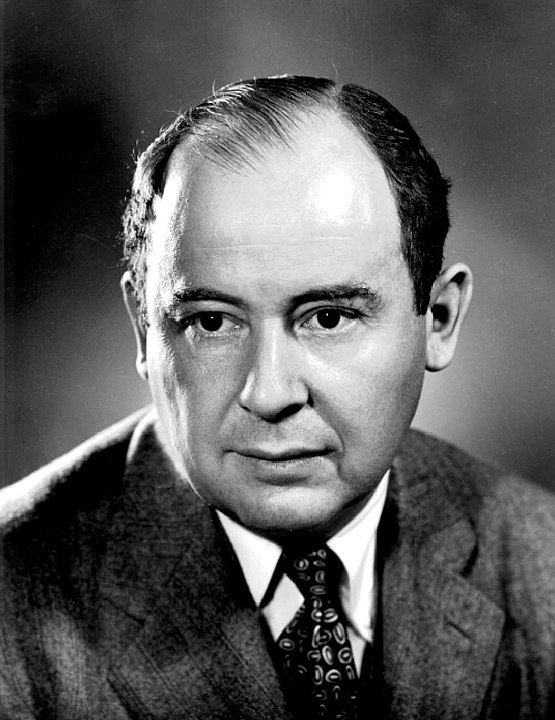
\includegraphics[width=0.2\textwidth]{fig/vonNeumann.png}
\end{center}
\begin{itemize}
\item 5 functional units – control unit, arithmetic logic unit, memory, input (devices), output (devices)
\item An computer architecture should be independent of solved problems. It has to provide mechanism to load program into memory. The program controls what the computer does with data, which problem it solves.
\item Programs and results/data are stored in the same memory. That memory consists of a cells of same size and these cells are sequentially numbered (address).
\item The instruction which should be executed next, is stored in the cell exactly after the cell where preceding instruction is stored (exceptions branching etc. ). 
\item The instruction set consists of arithmetics, logic, data movement, jump/branch and special/control instructions.
\end{itemize}
\end{frame}


\begin{frame}
\frametitle{Computer based on von Neumann's concept}

\begin{itemize}
\item Procesor/microprocessor
\begin{itemize}
\item Control unit
\item ALU
\end{itemize}
\item Memory - von Neumann architecture uses common memory, whereas Harvard architecture uses separate program and data memories
\item Input/output subsystem
\begin{itemize}
\item Input
\item Output
\end{itemize}
\end{itemize}
The control unit is responsible for control of the operation processing and sequencing. It consists of:
\begin{itemize}
\item registers – they hold intermediate and programmer visible state
\item control logic circuits which represents core of the control unit (CU)
\end{itemize}
\end{frame}


\begin{frame}
\frametitle{Registr FLAGS}
RFLAGS registr
\begin{center}
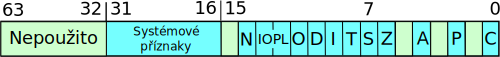
\includegraphics[width=0.65\textwidth]{flags-cz.pdf}
\end{center}
\begin{columns}[t,onlytextwidth]
\begin{column}{0.5\textwidth}
C -- Carry flag\\
P -- Parity flag\\
Z -- Zero flag\\
S -- Sign flag\\
O -- Overflow flag\\
A -- Auxiliary flag (BCD)
\end{column}
\begin{column}{0.5\textwidth}  
I -- Intterupt enable\\
T -- Trap flag\\
IOPL -- I/O privilege level\\
Systémové příznaky:
\begin{itemize}
\item VM -- Virtual 8086 Mode
\item VIF -- Virtual Interrupt Flag
\item VIP -- Virtual Interrupt Pending
\end{itemize}
\end{column}
\end{columns}
\end{frame}

\begin{frame}
\frametitle{Režimy práce procesoru}
FLAGS registr 
\begin{itemize}
  \item Dva režimy práce procesoru IOPL -- základ hardwarových ochran
  \begin{itemize}
    \item CPL0\footnote{Current privilege level} = privilegovaný (systémový) režim
    \begin{itemize}
      \item procesor může vše, čeho je schopen
    \end{itemize}
    \item CPL3 = uživatelský (aplikační) režim
    \begin{itemize}
      \item privilegované operace  jsou zakázány
    \end{itemize}
  \end{itemize}
  \item Privilegované operace
  \begin{itemize}
    \item ovlivnění stavu celého systému (halt, reset, Interrupt Enable/Disable, modifikace Flags,  modifikace registrů MMU ) 
    \item instrukce pro vstup/výstup (in, out)
  \end{itemize}

  \item Přechody mezi režimy
  \begin{itemize}
    \item Po zapnutí stroje systémový režim
    \item Přechod do uživatelského – modifikace Flags (popf nebo reti)
    \item Přechod do systémového – pouze přerušení vč. programového
  \end{itemize}
\end{itemize}
\end{frame}


\section{Instrukce x86}

\begin{frame}
\frametitle{Instrukce – x86/AMD64}
Instrukce ``ulož hodnotu''\\
(běžně se používají dvě různé syntaxe pro zápis assembleru)\\

\begin{tabular}{ l l }
\textbf{AT\&T} & \textbf{Intel}\\
\texttt{movq} zdroj 64b, cíl &	\texttt{mov} cíl, zdroj\\
\texttt{movl} zdroj 32b, cíl &\\
\texttt{movw} zdroj 16b, cíl &\\
\texttt{movb} zdroj 8b, cíl &\\
registry se značí &\\
\texttt{\%ax}	& pouze \texttt{ax}\\
hodnoty \$, hex 0x & číslo, hex postfix h\\
&\\
\texttt{movl \$0xff, \%ebx} & \texttt{mov ebx, 0ffh}\\
\end{tabular}
\end{frame}


\begin{frame}
\frametitle{Instrukce – x86/AMD64}
Načti hodnotu z adresy (odkaz do paměti)\\
\begin{tabular}{ l l}
AT\&T & Intel \\
\texttt{movl (\%ecx),\%eax} & \texttt{mov eax, [ecx]}\\
\texttt{movl 3(\%ebx), \%eax} & \texttt{mov eax, [ebx+3]} \\
\texttt{movl (\%ebx, \%ecx, 0x2), \%eax} & \texttt{mov eax, [ebx+ecx*2h]} \\
\texttt{movl -0x20(\%ebx, \%ecx, 0x4), \%eax} & \texttt{mov eax, [ebx+ecx*4h-20h]} \\
\end{tabular}

\begin{itemize}
\item odkaz má 4 složky: \emph{základ+index*měřítko+posun}
\item \emph{měřítko} může nabývat hodnot 1,2,4,8
\item lze implementovat přístup do pole struktur: \emph{základ} je ukazatel na první prvek, \emph{index*měřítko} říká, který prvek chceme a \emph{posun}, kterou položku uvnitř struktury potřebujeme.
\item není potřeba použít všechny 4 složky 
\end{itemize}
\end{frame}


\begin{frame}
\frametitle{Instrukce opakování – x86/AMD64}
Instrukce pro řetězce  - \texttt{REP} opakování pro pole hodnot
\begin{itemize}
\item opakuj dokud \texttt{ecx>0}:
\begin{itemize}
\item \texttt{operace (\%esi), (\%edi)}
\item \texttt{esi += d*operand\_size}
\item \texttt{edi += d*operand\_size}
\item \texttt{ecx - -}
\end{itemize}
\item operace může být \texttt{movs, cmps, lods, stos, scas, ins, outs}
\item \texttt{d} - určuje směr a je buď +1, nebo -1
\item \texttt{REP} opakování podle hodnoty \texttt{ecx}
\item \texttt{REPE/REPNE} opakování podle hodnoty \texttt{ecx} a podle porovnání
  \begin{itemize}
  \item operace \texttt{cmps} se navíc zastaví, pokud je/není rozdíl mezi \texttt{(edi)} a \texttt{(esi)} 
  \item operace scas se navíc zastaví, pokud je/není rozdíl mezi \texttt{(edi)} a hodnotou v registru \texttt{eax} 
  \end{itemize}
\end{itemize}

\end{frame}


\begin{frame}[fragile]
\frametitle{Instrukce opakování – x86/AMD64}
Příklad nastav pole na hodnotu -1:
\begin{lstlisting}[language={C},columns=flexible]
int array[128];
for (int i=0; i<128; i++) {array[i]=-1;}
\end{lstlisting}
přeloženo:
\begin{lstlisting}[language={[x86masm]Assembler},columns=flexible]
mov   array, %edi  ; Nastav do edi ukazatel na zacatek pole
mov   $128,  %ecx  ; Nastav pocet opakovani
mov   $-1,   %eax  ; Nastav hodnotu pro ulozeni
rep stosd          ; Vypln cele pole
\end{lstlisting}
\end{frame}

\begin{frame}[fragile]
\frametitle{Instrukce opakování – x86/AMD64}

Najdi konec řetězce:
\begin{lstlisting}[language={C},columns=flexible]
char str[128];
int i;
for (i=0; i<128; i++) {if (str[i]==0) break;}
\end{lstlisting}
přeloženo:
\begin{lstlisting}[language={[x86masm]Assembler},columns=flexible]
mov   str,  %edi  ; Nastav do EDI zacattek pole
mov   $128, %ecx  ; Nastav pocet opakovani
mov   $0,   %eax  ; Nastav hodnotu konce retezce
rep scasb         ; Projdi str a najdi 0 hodnotu
\end{lstlisting}

\end{frame}



\begin{frame}
\frametitle{Instrukce – x86/AMD64}
Aritmetika -- AT\&T syntax
\begin{tabular}{ l l}
operace co, k čemu &\\
\texttt{addq    \$0x05,\%rax} & rax = rax + 5\\
\texttt{subl    -4(\%ebp), \%eax} &  eax = eax -- mem(ebp-4)\\
\texttt{subl    \%eax, -4(\%ebp)} & mem(ebp-4) = mem(ebp-4)-eax\\
\multicolumn{2}{l}{následující instrukce mají argumenty typu X -- b, w, l, q}\\
\texttt{andX} & bitový and\\
\texttt{orX} & bitový or\\
\texttt{xorX} & bitový xor (nejrychlejší vynulování registru)\\
\texttt{mulX} & násobení čísel bez znamének\\
\texttt{divX} & dělení čísel bez znamének\\
\texttt{imulX} & násobení čísel se znaménky\\
\texttt{idivX} & dělení čísel se znaménky\\
\end{tabular}
\end{frame}

\begin{frame}
\frametitle{Instrukce – x86/AMD64}
Aritmetika s jedním operandem -- AT\&T syntax
\begin{tabular}{ l l}
operace   s cim&\\
\texttt{incl            \%eax} &              eax = eax + 1\\
\texttt{decw            (\%ebx)} &                 mem(ebx) = mem(ebx)-1\\
\texttt{shlb            \$3, \%al} &                al = al$<<$3\\
\texttt{shrb            \$1, \%bl} &                bl=11000000, po bl=01100000\\
\texttt{sarb            \$1, \%bl} &                bl=11000000, po bl=11100000\\
\texttt{rorx, rolx} & bitová rotace doprava a doleva\\
\texttt{rcrx, rcl} & bitova rotace – pres C -- carry flag\\
\end{tabular}
\end{frame}


\begin{frame}
\frametitle{Instrukce – x86/AMD64}
Podmíněné skoky\\
\begin{tabular}{ l l}
\texttt{test    a1, a2} &  tmp = a1 AND a2, Z tmp=0, C tmp<0\\
\texttt{cmp     a1, a2} &  tmp = a1-a2, Z tmp=0, C tmp<0\\
\end{tabular}

pak lze použít následující skoky
\begin{tabular}{ l l}
\texttt{jmp kam} & nepodmíněný skok, vlastně \texttt{\%eip=kam}\\
\texttt{je      kam} & jmp equal -- skoč při rovnosti\\
\texttt{jne kam} & jmp not equal -- skoč při nerovnosti\\
\texttt{jg/ja kam} & jmp greater – skoč pokud je a1 > a2 (sign/unsig)\\
\texttt{jge/jae kam} & skoč pokud je a1 >= a2 (sign/unsig)\\
\texttt{jl/jb kam} & jmp less – skoč pokud je a1 < a2 (sign/unsig)\\
\texttt{jle/jbe kam} & skoč pokud je a1 <= a2 (sign/unsig)\\
\texttt{jz/jnz kam} & skoč pokud je Z=1/0\\
\texttt{jo/jno kam}& skoč pokud je O (overflow) = 1/0\\
\end{tabular}
\end{frame}

\begin{frame}
\frametitle{Quiz}
Liší se velikost programů pro CISC (x86) a RISC (RISC V)?
\begin{itemize}
\item[A] neliší, je přibližně stejná
\item[B] programy pro CISC jsou delší
\item[C] programy pro RISC jsou delší
\end{itemize}

\end{frame}


\begin{frame}[fragile]
\frametitle{Porovnání CISC vs. RISC}
CISC programy jsou kratší:
\begin{lstlisting}[language={[x86masm]Assembler},columns=flexible]
incl 10(%ecx)      =      lw   t2, 10(t1)
                          addi t2, t2, 1
                          sw   t2, 10(t1)

rep movs           = l1:  lw   t3, 0(t1) 
                          sw   t3, 0(t2)
                          addi t1, t1, 4
                          addi t2, t2, 4
                          addi t4, t4, -1
                          jne  t4, zero, l1 
\end{lstlisting}

\end{frame}

\begin{frame}
\frametitle{Quiz}
Jsou prgramy pro CISC (x86) rychlejší než pro RISC (RISC V)?
\begin{itemize}
\item[A] Ano 
\item[B] Ne
\item[C] Jak kdy, záleží na procesoru
\end{itemize}

\end{frame}



\begin{frame}
\frametitle{Zásobník}

\begin{columns}
\begin{column}{0.45\textwidth}
Zásobník:
\begin{itemize}
\item obecná struktura LIFO
\item operace push vloží data do zásobníku
\item operace pop vybere data ze zásobníku
\end{itemize}
\begin{center}
   
\includegraphics[width=0.5\textwidth]{stack.pdf}
\end{center}

\end{column}

\begin{column}{0.55\textwidth}  
Implemetace:
\begin{itemize}
\item implementace registrem \textit{SP} - ukazuje na vrchol zásobníku
\item konvence - při každém pop se zvětšuje registr \textit{SP} o velikost operandu, při push se \textit{SP} zmenšuje.
\end{itemize}
\begin{tabular}{ l l}
\texttt{pushl \%eax} &  ulož eax na zásobník\\
\texttt{popw \%bx}   &  vyber ze zásobníku \\
                     &  2 bajty do \textit{bx}\\
\texttt{pushf/popf}  &  ulož/vyber register\\
                     &  EFLAGS\\
\texttt{pusha/popa}  &  ulož/vyber všechny\\
                     &  uživatelské registry\\
\end{tabular}
\end{column}
\end{columns}
\end{frame}


\begin{frame}[fragile]
\frametitle{Quiz}

Mějme program:
\begin{columns}
\begin{column}{0.45\textwidth}
\begin{lstlisting}[language={C},columns=flexible]
int factorial(int x) {
  int y;
  if (x<=1) {
    return 1;
  } else {
    y = factorial(x-1)
    return y*x;
  }
}
\end{lstlisting}
\end{column}
\hfill
\begin{column}{0.45\textwidth}  
\begin{lstlisting}[language={C},columns=flexible]
int i;
int main() {
  i=10;
  i=factorial(i);
  return i;
}
\end{lstlisting}
\end{column}
\end{columns}

Kde se bude nacházet proměnná i?
\begin{itemize}
\item[A] Pro RISC V i pro x86 na zásobníku
\item[B] Pro RISC V dynamicky alokovaná, pro x86 na zásobníku
\item[C] Pro RISC V i pro x86 na místě v paměti určeném při překladu
\item[D] Pro RISC V i pro x86 nelze uričit
\end{itemize}
\end{frame}


\begin{frame}[fragile]
\frametitle{Quiz}

Mějme program:
\begin{columns}
\begin{column}{0.45\textwidth}
\begin{lstlisting}[language={C},columns=flexible]
int factorial(int x) {
  int y;
  if (x<=1) {
    return 1;
  } else {
    y = factorial(x-1)
    return y*x;
  }
}
\end{lstlisting}
\end{column}
\hfill
\begin{column}{0.45\textwidth}  
\begin{lstlisting}[language={C},columns=flexible]
int i;
int main() {
  i=10;
  i=factorial(i);
  return i;
}
\end{lstlisting}
\end{column}
\end{columns}

Kde se bude nacházet proměnná y při překladu bez optimalizace?
\begin{itemize}
\item[A] Pro RISC V i pro x86 na zásobníku
\item[B] Pro RISC V i pro x86 dynamicky alokovaná
\item[C] Pro RISC V i pro x86 na místě v paměti určeném při překladu
\item[D] Pro RISC V i pro x86 nelze uričit
\end{itemize}
\end{frame}

\begin{frame}[fragile,shrink=10]
\frametitle{Quiz}

Mějme program:
\begin{columns}
\begin{column}{0.45\textwidth}
\begin{lstlisting}[language={C},columns=flexible]
int factorial(int x) {
  int y;
  if (x<=1) {
    return 1;
  } else {
    y = factorial(x-1)
    return y*x;
  }
}
\end{lstlisting}
\end{column}
\hfill
\begin{column}{0.45\textwidth}  
\begin{lstlisting}[language={C},columns=flexible]
int i;
int main() {
  i=10;
  i=factorial(i);
  return i;
}
\end{lstlisting}
\end{column}
\end{columns}

Kde se bude nacházet proměnná x při překladu bez optimalizace?
\begin{itemize}
\item[A] Pro RISC V i pro x86 na zásobníku
\item[B] Pro RISC V v registru, pro x86 na zásobníku
\item[C] Pro RISC V v registru a následně bude uložena na zásobník, pro x86 na zásobníku
\item[D] Pro RISC V na zásobníku, pro x86 v registru
\item[E] Pro RISC V na zásobníku, pro x86 v registru a následně na zásobníku
\end{itemize}
\end{frame}

\begin{frame}[fragile,shrink=10]
\frametitle{Quiz}

Mějme program:
\begin{columns}
\begin{column}{0.45\textwidth}
\begin{lstlisting}[language={C},columns=flexible]
int factorial(int x) {
  int y;
  if (x<=1) {
    return 1;
  } else {
    y = factorial(x-1)
    return y*x;
  }
}
\end{lstlisting}
\end{column}
\hfill
\begin{column}{0.45\textwidth}  
\begin{lstlisting}[language={C},columns=flexible]
int i;
int main() {
  i=10;
  i=factorial(i);
  return i;
}
\end{lstlisting}
\end{column}
\end{columns}

Kde se bude nacházet návratová adresa z funkce factorial?
\begin{itemize}
\item[A] Pro RISC V i pro x86 na zásobníku
\item[B] Pro RISC V v registru, pro x86 na zásobníku
\item[C] Pro RISC V v registru a následně bude uložena na zásobník, pro x86 na zásobníku
\item[D] Pro RISC V na zásobníku, pro x86 v registru
\item[E] Pro RISC V na zásobníku, pro x86 v registru a následně na zásobníku
\end{itemize}
\end{frame}


\begin{frame}
\frametitle{Funkce zásobníku}

Zásobník:
\begin{itemize}
  \item parametry pro funkci
  \item kam se vrátit po ukončení funkce, místo odkud program volal funkci
  \item lokální proměnné funkce
  \begin{itemize}
    \item zásobník je vetšinou malý
    \item omezená velikost lokálních proměnných
    \item pozor při rekurzi - lépe se rekurzi vyhnout
  \end{itemize}
\end{itemize}

\end{frame}


\begin{frame}[fragile]
\frametitle{Instrukce – x86/AMD64}
Volání funkce\\
\begin{tabular}{ l l}
\texttt{call adr} &         vlastně \texttt{push \%eip}, \texttt{jmp adr}\\
\texttt{ret} &              vlastně \texttt{pop \%eip}\\
\texttt{leave} &            vlastně \texttt{mov \%ebp, \%esp} a \texttt{pop \%ebp}\\
\end{tabular}\\
\bigskip
Lokální proměnné ve funkci – příklad implementace
\begin{lstlisting}[language={[x86masm]Assembler},columns=flexible]
push  %ebp        ; Ulozime hodnotu EBP do zasobniku
mov   %esp, %ebp  ; Zkopirujeme hodnotu registru ESP to EBP
sub   $12, %esp   ; Snizime ukazatel zasobniku o 3x4 bajty
\end{lstlisting}
První proměnná bude na adrese \texttt{-4(\%ebp)}, druha \texttt{-8(\%ebp)}\\
První parametr bude na adrese \texttt{8(\%ebp)}, další \texttt{12(\%ebp)}

\begin{lstlisting}[language={[x86masm]Assembler},columns=flexible]
mov   %ebp, %esp  ; Vratime ukazatel zpet na puvodni pozici.
pop   %ebp        ; Obnovime puvodni hodnotu registru EBP
ret               ; Navrat z funkce
\end{lstlisting}
\end{frame}


\begin{frame}
\frametitle{Instrukce – x86/AMD64}
Složitost assembleru
\begin{itemize}
\item Algoritmus se dá přeložit různými způsoby do assembleru
\item Strojový překlad je někdy hodně kostrbatý
\begin{itemize}
\item např. \texttt{mov 0x12345, \%esi; mov \%esi, \%ebx} místo \texttt{mov 0x12345, \%ebx}
\end{itemize}
\item Různé způsoby pracují různě rychle a jsou rozdílně dlouhé a rozdílně přehledné
\begin{itemize}
\item \texttt{xor \%ebx, \%ebx}  je to samé jako \texttt{ mov \$0, \%ebx}
\item \texttt{lea} adresa, registr – load effective address – nastaví hodnotu ukazatele do zadaného registru
\item \texttt{lea   -12(\%esp), \%esp }  je to samé jako \texttt{ sub    \$12, \%esp} 
\item lea je výhodnější vzhledem k předzpracování instrukcí, nezatěžuje ALU jednotku (ovšem třeba Atom má zpracování adr. pomalejší než ALU).
\end{itemize}
\end{itemize}
\end{frame}

\section{FPU - x87}


\begin{frame}
\frametitle{FPU coprocesor – x87}
Speciální součást procesoru pro práci s reálnými čísly
\begin{itemize}
\item Podporuje single-32, double-64, extended-80 i exotické formáty BCD
\item Obsahuje vlastních 8 registrů o 80 bitech
\item Registry jsou organizovány v zásobníku (push, pop), ale umožňují i přímý přístup (0-7)
\item Každá operace pracuje s vrcholem zásobníku a jedním dalším registrem, nebo hodnotou
\item Původně oddělený procesor, od 486 on-die -- na jednom čipu
\item Podporuje všechny IEEE-754 operace:
\begin{itemize}
\item fadd, fsub, fmul, fdiv, fsqrt, fcmp, fsin, ...
\end{itemize}
\end{itemize}
\end{frame}

\begin{frame}
\frametitle{Způsob práce FPU}
Základní operace slouží pro uložení reálného čísla z/do registrů:
\begin{itemize}
\item fld - uloží hodnotu z paměti na zásobník registrů -- push
\item fst - uloží hodnotu z registru do paměti bez pop
\item fstp - uloží hodnotu z registru do paměti a udělá pop
\end{itemize}
Základní operace pro uložení celého čísla (integer) z/do registrů:
\begin{itemize}
\item fild - uloží celé číslo z paměti na zásobník registrů -- push
\item fist - uloží celé číslo z registru do paměti bez pop
\item fistp - uloží celé číclo z registru do paměti a udělá pop
\item fisttp - uloží zaokrouhlené celé číclo z registru do paměti a udělá pop
\end{itemize}
\end{frame}

\begin{frame}
\frametitle{Operace FPU}
Práci základních operací si ukážeme na sčítání (ostatní oprace mají shodný tvar, ST(0) je vrchol zásobníku, ST(1) hodnota pod ním, atd.):
\begin{itemize}
\item fadd float/double - přičti obsah paměti k ST(0) a výsledek ulož do ST(0)
\item fiadd short/int - přičti celé číslo z paměti k ST(0) a výsledek ulož do ST(0)
\item fadd ST(0), ST(i) - sečti obsah ST(0) a ST(i) a výsledek ulož do ST(0)
\item fadd ST(i), ST(0) - sečti obsah ST(i) a ST(0) a výsledek ulož do ST(i)
\item faddp ST(i), ST(0) - sečti obsah ST(i) a ST(0) a výsledek ulož do ST(i) a udělej pop operaci (zruš hodnotu ST(0))
\item faddp - sečti obsah ST(1) a ST(0) a výsledek ulož do ST(1) a udělej pop operaci (zruš hodnotu ST(0))
\end{itemize}
\end{frame}


\begin{frame}
\frametitle{Operace FPU}
Operace SUB a DIV mají navíc i reverzní formu, tedy otočení pořadí operandů (ve všech verzích, jak s pamětí, tak s registry):
\begin{itemize}
\item fsub ST(0), ST(i) - výsledek ST(0) - ST(i) ulož do ST(0)
\item fsubr ST(0), ST(i) - výsledek ST(i) - ST(0) ulož do ST(0)
\end{itemize}

Unární funkce sin, cos:
\begin{itemize}
\item fsin/fcos - ST(0) nahraď hodnotou sin/cos(ST(0))
\end{itemize}

Logaritmus - výpočet $y\cdot\log_2 x$:
\begin{itemize}
\item fyl2x - ST(1) nahraď hodnotou ST(1)*($log_2$ ST(0)) a udělej pop
\end{itemize}

Načtení konstant:
\begin{itemize}
\item fldz/fld1 - uloží 0.0/1.0 na zásobník 
\item fldpi/fldl2e - uloží $\pi$/$\log_2 e$ na zásobník 
\end{itemize}

\end{frame}


\begin{frame}[fragile]
\frametitle{Příklad programu s FPU}
Příklad výpočtu 1.1*2.2+sin(3.3):
\begin{lstlisting}[language={[x86masm]Assembler},columns=flexible]
fldl   adr_1.1  ; Nacteme prvni operand
fmull  adr_2.2  ; Vynasobime prvni op druhym op
fldl   adr_3.3  ; Nacteme treti operand
fsinl           ; Spocti sin tretiho operandu
faddp           ; Secti dve cisla a ponech jen soucet
fstp   adr_vysl ; Uloz vysledek do pameti
\end{lstlisting}

\end{frame}


\begin{frame}
\frametitle{FPU pro RISC V}
\begin{itemize}
\item Dvě rozšíření RV64F – float, RV64D – double
\item 32 interních registrů, buď o velikosti 32 bitů pro float, nebo o velikosti 64 bitů pro double
\item Nové instrukce pro načtení load a store – flw, fsw (fld, fsd)
\item Nové instrukce pro operace:
\begin{itemize}
\item fadd.s, fsub.s, fmul.s, fdiv.s ( *.d pro double)
\item fadd.s   F[rd]=F[rs1]+F[rs2] 
\item fsqrt.s -- square root -- odmocnina  F[rd] = sqrt(F[rs1])
\item fmadd.s -- násob a sečti, F[rd]=F[rs1]*F[rs2]+F[rs3]
\item fmsub.s -- násob a odečti, F[rd]=F[rs1]*F[rs2]-F[rs3]
\item fmin.s -- F[rd] = (F[rs1]<F[rs2]) ? F[rs1] : F[rs2]
\item převody mezi float, double a celými čísly
\end{itemize}
\end{itemize}
\end{frame}

\section{Rozšíření MMX}


\begin{frame}
\frametitle{SIMD - MMX}

\begin{itemize}
\item SIMD - Single Instruction Multiple Data - provedení jednoho typu instrukce na více datech najednou
\item MMX - MultiMedia eXtension (někdy se vysvětluje jako Multiple Math eXtension)
\item Využívají stejné registry jako FPU x87, nelze je tedy používat současně
\item 64-bitový registr může fungovat v následujících módech:
\begin{itemize}
\item B - $8\times$ bajt
\item W - $4\times$ short int
\item D - $2\times$ int
\end{itemize}
\item Operace: 
\begin{itemize}
\item Aritmetické - sčítání, odčítání, násobení
\item Logické - and, or, rotace, porovnání
\item Konverze - pack, přesuny mezi registry
\end{itemize}
\end{itemize}
\end{frame}

\begin{frame}
\frametitle{MMX operace}
\begin{columns}[t,onlytextwidth]
  \begin{column}{0.5\textwidth}
    \texttt{PADDW} - součet po částech (packed)
  \end{column}
  \begin{column}{0.5\textwidth}
    \texttt{PADDUSW} - součet saturovaný (bez přetečení)
  \end{column}
\end{columns}
\begin{columns}[t,onlytextwidth]
  \begin{column}{0.5\textwidth}
    \begin{center}
    
\includegraphics[width=0.8\textwidth]{mmx-add.pdf}
    \end{center}
  \end{column}
  \begin{column}{0.5\textwidth}
    \begin{center}
    
\includegraphics[width=0.8\textwidth]{mmx-add-sat.pdf}
    \end{center}
  \end{column}
\end{columns}

\end{frame}

\begin{frame}
\frametitle{MMX operace}
\small
    \begin{center}
    \texttt{PMADDWD} - vynásob a sečti\\
    
\includegraphics[width=0.4\textwidth]{mmx-mul-add.pdf}
    \end{center}
\vspace{-1cm}
\begin{columns}[t,onlytextwidth]
  \begin{column}{0.5\textwidth}
    \begin{center}
    \texttt{PMULLW} - součin (spodní část)
    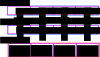
\includegraphics[width=0.8\textwidth]{mmx-mull.pdf}
    \end{center}
  \end{column}
  \begin{column}{0.5\textwidth}
    \begin{center}
    \texttt{PMULHW} - součin (vrchní část)
    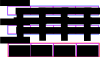
\includegraphics[width=0.8\textwidth]{mmx-mulh.pdf}
    \end{center}
  \end{column}
\end{columns}


\end{frame}


\begin{frame}[fragile]
\frametitle{MMX příklad}

\begin{columns}[t,onlytextwidth]
  \begin{column}{0.5\textwidth}
Maskování obrazu v obraze:
\begin{lstlisting}[language={C},columns=flexible]
unsigned char mask[size],
 obr1[size], obr2[size];
if (mask[i]==0) {
  new_img[i] = obr1[i];
} else {
  new_img[i] = obr2[i];
}
\end{lstlisting}

  \end{column}
  \begin{column}{0.5\textwidth}
MMX implementace 8 pixelů najednou
\begin{lstlisting}[language={[x86masm]Assembler},columns=flexible]
movq    mask_ptr, %mm0
pcmpeqb %mm0, 0
movq    %mm0, %mm1
pand    %mm1, obr1_ptr
pandn   %mm0, obr2_ptr
por     %mm0, %mm1
movq    %mm0, new_img_ptr
\end{lstlisting}
  \end{column}
\end{columns}
\end{frame}




\begin{frame}
\frametitle{3Dnow! rozšíření MMX}
\begin{itemize}
\item Rozšíření 3Dnow! přidalo ve stávajících registrech \texttt{mm0}-\texttt{mm7} práci s reálnými čísly. 
\item Umožňuje pouze dělení registru na dvě reálná čísla po 32bitech
\item Přidává konverzi celých čísel na reálná čísla a zpět, také pomocí průměrování 8-bitových a 16-bitových celých čísel
\item Sčítání, odčítání, násobení, dělení reálných čísel po složkách
\item Porovnávání reálných čísel a nalezení minim a maxim
\end{itemize}
\end{frame}

\section{Rozšíření SSE}


\begin{frame}
\frametitle{SSE další SIMD}
\begin{itemize}
\item SSE - Streaming SIMD Extension
\item nové registry xmm0-xmm7
\item každý registr 128-bitů, možné dělení
\item $4\times$ float - 32-bitové reálné číslo
\item $2\times$ double - 64-bitové reálné číslo
\item rozšíření celočíselných operací MMX na 128-bitové registry
\end{itemize}
\end{frame}



\begin{frame}
\frametitle{Instrukce SSE}
\begin{itemize}

\item Operace: packet suffix -ps, scalar suffix -ss 



\item Uložit z/do paměti: mov
\item Aritmetické operace float: add, sub, mul, div, rcp, sqrt, max, min, rsqrt
\item Logické operace: and, or, xor, andn
\item Porovnání: cmp, comi, ucomi


\item Scalar operation: addss, subss, mulss, divss
\end{itemize}
\end{frame}

\begin{frame}
\frametitle{Packet SSE}
\begin{columns}[t,onlytextwidth]
\begin{column}{0.5\textwidth}
\begin{center}
Packet operation

\includegraphics[width=0.9\textwidth]{sse.pdf}
\end{center}
\end{column}
\begin{column}{0.5\textwidth}
\begin{center}
Scalar operation

\includegraphics[width=0.9\textwidth]{sse-s.pdf}
\end{center}
\end{column}
\end{columns}
\end{frame}

\begin{frame}
\frametitle{Rozšíření SSE}
Další rozšíření:
\begin{itemize}
\item SSE2 - přidala dalších 144 nových instrukcí
\item SSE3 - dalších 13 instrukcí
\item SSSE3 - dalších 16 instrukcí
\item SSE4 - dalších 47 nových instrukcí
\item SSE4.2 - dalších 170 nových instrukcí
\end{itemize}
\end{frame}


\end{document}

